\section{Preliminaries}
\label{sec:prelim}

This section states the mobile-UWSN architecture and the acoustic,
multipath, noise, and Q-learning objects that E-LQTP inherits from
LQARP \cite{liu2026lqarp}.
The inherited objects are restated so that the dual-track estimator
of Section~\ref{sec:design} can be written against a closed system
model; no new channel or learning contribution is claimed.
Subsection~\ref{sec:prelim:est} isolates the estimation problem that
mobility adds on top of that foundation.

\subsection{Network Architecture}
\label{sec:prelim:arch}
\begin{figure*}[!t]
\centering
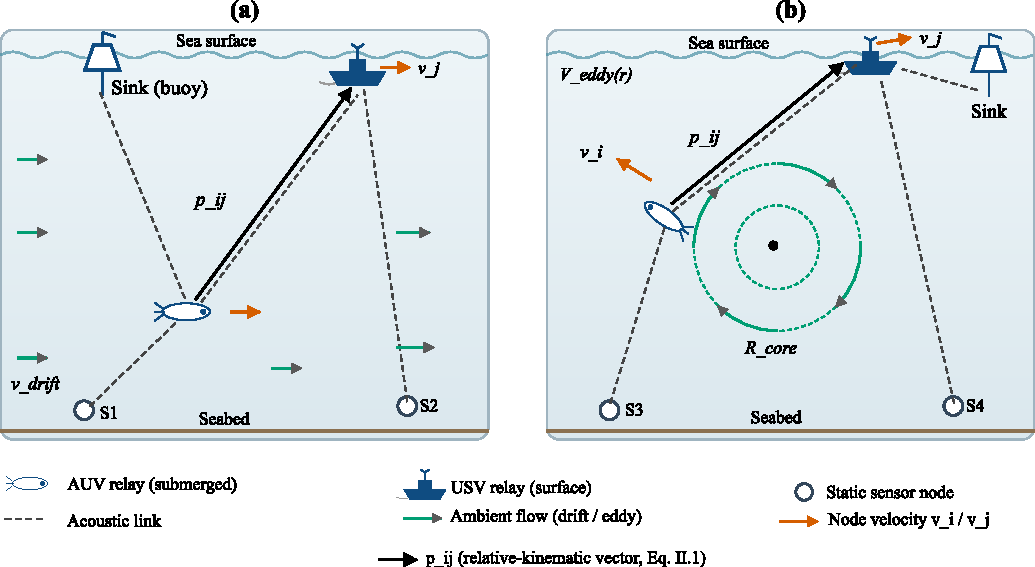
\includegraphics[width=\textwidth]{elqtp_figs/fig1_network_architecture}
\caption{Mobile UWSN. (a)~Shared current. (b)~Rankine eddy.
Solid: relative kinematic vector $p_{ij}$. Dashed: acoustic link.}
\label{fig:network_architecture}
\end{figure*}

The network is a single-sink acoustic mesh of $N$ autonomous
underwater vehicles (AUVs) and one unmanned surface vehicle (USV)
sink, deployed in a
$L\times L\times H=6\,\mathrm{km}\times 6\,\mathrm{km}\times
500\,\mathrm{m}$ Western Pacific water column
(Fig.~\ref{fig:network_architecture}).
The sink sits at the horizontal centroid with kinematic depth
$z_{\mathrm{sink}}=5\,\mathrm{m}$, so that it is uniquely shallowest
for the depth-progressive candidate filter of
Section~\ref{sec:prelim:q}.
Its acoustic query depth is independent of that kinematic depth and
is set to the Bellhop source-depth slice $z_{\mathrm{ac}}=50\,\mathrm{m}$
(a towed or hull-offset transducer).
Each AUV $s_i$ has kinematic state
$(p_i,\dot{p}_i)\in\mathbb{R}^3\times\mathbb{R}^3$, residual energy
$E_{s_i}$, and a feasible-neighbor count $\mathrm{number}_{s_i}$.
Relays are placed uniformly in
$[0,L]^2\times[10,H]$ with a $1\,\mathrm{m}$ three-dimensional
separation floor.
The sink does not generate data.
Every AUV emits a data packet of $l=400\,\mathrm{bit}$ every
$30\,\mathrm{s}$.

Two mobility fields are used in evaluation
(Fig.~\ref{fig:network_architecture}) and are drawn at $N=40$ in
Fig.~\ref{fig:mobility_fields}.
Scenario~I is the stationary identity:
$\dot{p}_i\equiv 0$.
Scenario~II is a shared horizontal current
$\dot{p}_i(t)=v_{\mathrm{cmd},i}+v_{\mathrm{drift}}$ with
$v_{\mathrm{cmd},i}=0$ and $\dot{p}_{\mathrm{sink}}=0$, so that
AUV--AUV relative velocity is identically zero and the only
persistent range-rate is AUV-to-sink.
Scenario~III replaces the uniform current with a counterclockwise
Rankine eddy centered on the sink plus an independent horizontal
Gauss--Markov fluctuation, so that AUV--AUV $v_{\mathrm{rel}}$ is
nonzero.
A relay that leaves the valid horizontal envelope is removed;
in-flight packets at that node fail as envelope-exit losses, not voids.
Vertical current is not modelled: a $1\,\mathrm{m/s}$ vertical
component would empty the $500\,\mathrm{m}$ column in a few hundred
seconds.

\subsection{Underwater Acoustic Channel}
\label{sec:prelim:urick}
Instantaneous link quality is the sonar-equation SNR on a
precomputed Bellhop field, inherited from LQARP
\cite{liu2026lqarp}.
For a transmitter--receiver pair $(s_i,s_j)$,
\begin{equation}
\label{eq:snr}
\mathrm{SNR}(s_i,s_j)
= \mathrm{SL}-\mathrm{TL}(r_H,z_q)-\mathrm{NL}+\mathrm{DI},
\end{equation}
where $\mathrm{SL}=175\,\mathrm{dB}$ re $1\,\mu\mathrm{Pa}@1\,\mathrm{m}$
is the source level, $\mathrm{DI}=0\,\mathrm{dB}$ is the
omnidirectional directivity index, and $\mathrm{NL}$ is the
band-integrated Wenz level of Section~\ref{sec:prelim:noise}.
Horizontal range $r_H=\|(x_i-x_j,y_i-y_j)\|$ and query depth
$z_q=\max(z_j^{\mathrm{ac}},5\,\mathrm{m})$ index a January
World Ocean Atlas 2023 / GEBCO cell at
$20.125^\circ\mathrm{N}$, $124.125^\circ\mathrm{E}$
(seafloor $5524\,\mathrm{m}$, source depth $50\,\mathrm{m}$,
carrier $24\,\mathrm{kHz}$, integration band $B=2\,\mathrm{kHz}$).
Transmission loss is the sonar-equation column of that grid,
\begin{equation}
\label{eq:tl}
\mathrm{TL}(r_H,z_q)=-10\log_{10}\bar{G}(r_H,z_q),
\end{equation}
with $\bar{G}$ the in-band power average of the equivalent transfer
function reconstructed from Bellhop eigenrays (geometric spreading
with $\kappa=2$ and Thorp absorption as in LQARP
\cite{liu2026lqarp}; Bellhop amplitudes are not reused, so spreading
and absorption are not double-counted).
A lookup that is non-finite is treated as a failed link:
$\mathrm{SNR}\ge\mathrm{SNR}_{\mathrm{th}}=8.68\,\mathrm{dB}$ is
reception, and any non-finite or sub-threshold value is a failed link.
The January $50\,\mathrm{m}$ crossing range at that threshold is
$r_{\mathrm{range}}=5125\,\mathrm{m}$.
Every protocol variant---LQARP, E-LQTP, the RLOR-inspired baseline,
and the Fixed-Periodic ablation---uses the same Bellhop lookup for
every SNR decision \cite{liu2026lqarp}.

\subsection{Multipath Representation}
\label{sec:prelim:mp}
The channel is frequency-selective on this site.
Water-column delay spread of about $3\,\mathrm{ms}$ at $1\,\mathrm{km}$
sets a coherence bandwidth of a few hundred hertz, much narrower
than $B=2\,\mathrm{kHz}$.
The scalar used by routing is therefore the $2\,\mathrm{kHz}$
power average $\bar{G}$, not a single-frequency coherent snapshot.
That average is the LQARP-style link budget; it does not resolve
fast fading, and the median pre-filter of
Section~\ref{sec:design:ekf} is not claimed to do so either.
Out-of-envelope (range, depth) cells are stored as non-finite and
are rejected by the reception gate rather than interpolated.

\subsection{Ambient Noise}
\label{sec:prelim:noise}
Ambient noise follows the four-component Wenz model inherited from
LQARP \cite{liu2026lqarp} at shipping factor $s=0.2$ and wind
$w=2.0\,\mathrm{m/s}$ (assumed, not taken from WOA/GEBCO).
The band-integrated level over $23$--$25\,\mathrm{kHz}$ is
$\mathrm{NL}=65.77\,\mathrm{dB}$ re $1\,\mu\mathrm{Pa}$.
At $24\,\mathrm{kHz}$ the spectral densities (dB re
$1\,\mu\mathrm{Pa}^2/\mathrm{Hz}$) are turbulence $-24.4$,
shipping $-13.0$, wave $32.7$, and thermal $12.6$; wind and thermal
terms dominate.
$\mathrm{NL}$ is constant on the grid; motion enters
\eqref{eq:snr} only through $\mathrm{TL}(r_H,z_q)$.

\subsection{Q-learning Routing}
\label{sec:prelim:q}
LQARP treats each node $s_i$ as a Q-learning agent
\cite{liu2026lqarp} on the MDP $(S,A,P,R)$.
The action $a_j$ selects neighbor $s_j$ as next hop.
A neighbor is a candidate only if it lies in all three of
\begin{align}
\label{eq:cand}
N_{\mathrm{range}}(s_i)
&= \{s_j:d(s_i,s_j)<r_{\mathrm{range}}\},\nonumber\\
N_{\mathrm{SNR}}(s_i)
&= \{s_j:\mathrm{SNR}(s_i,s_j)>\mathrm{SNR}_{\mathrm{th}},\,j\neq i\},\nonumber\\
N_{\mathrm{depth}}(s_i)
&= \{s_j:\mathrm{depth}_{s_i}-\mathrm{depth}_{s_j}>0,\,j\neq i\},
\end{align}
so that
$I(s_i)=N_{\mathrm{range}}(s_i)\cap N_{\mathrm{SNR}}(s_i)\cap
N_{\mathrm{depth}}(s_i)$ and $A=I(s_i)$.
The reward on a feasible action is
\begin{equation}
\label{eq:reward_lqarp}
R^{a_j}_{s_i,s_j}
= \frac{c_{\mathrm{ene}}(s_j)\,c_{\mathrm{del}}(s_i,s_j)\,
c_{\mathrm{nei}}(s_j)}{c_{\mathrm{lin}}(s_i,s_j)},
\end{equation}
with
\begin{align}
\label{eq:factors}
c_{\mathrm{lin}}(s_i,s_j)
&= \ln\!\bigl(1/P_{\mathrm{succ}}(s_i,s_j)\bigr),\nonumber\\
P_{\mathrm{succ}}
&= (1-p_e)^l,\nonumber\\
c_{\mathrm{ene}}(s_j)
&= (2/\pi)\arctan\bigl((E_{s_j}-E_{\mathrm{avg}})/E_{\mathrm{ini}}\bigr),\nonumber\\
c_{\mathrm{del}}(s_i,s_j)
&= (E_{s_j}/E_{\mathrm{ini}})\,
(\mathrm{depth}_{s_i}-\mathrm{depth}_{s_j}),\nonumber\\
c_{\mathrm{nei}}(s_j)
&= \exp(\mathrm{number}_{s_j}).
\end{align}
$p_e$ is the $M=2$ (BPSK) OFDM bit-error expression of LQARP
Eq.~34, floored at $p_e=\max(p_e^{\mathrm{AWGN}},10^{-9})$ so that
$c_{\mathrm{lin}}$ remains finite on the high-SNR plateau that is
typical at short range on this grid
($c_{\mathrm{lin}}\approx 4\times 10^{-7}$ for $l=400$).
$E_{\mathrm{avg}}$ is the mean residual energy over $I(s_i)$, not
the global mean; $\mathrm{number}_{s_j}=|I(s_j)|$, and
$c_{\mathrm{nei}}=1$ when $s_j$ has no onward candidate.
The temporal-difference update is
\begin{equation}
\label{eq:q}
Q(s_i,a_j)
\leftarrow (1-\alpha)Q(s_i,a_j)
+\alpha\Bigl[R^{a_j}_{s_i,s_j}
+\gamma\max_{a\in I(s_j)}Q(s_j,a)\Bigr],
\end{equation}
with $\alpha=0.9$, $\gamma=0.8$, and
$s_i.\mathrm{NextHop}=\arg\max_{a_j\in I(s_i)}Q(s_i,a_j)$.
Q-values start at zero.

When $I(s_i)=\emptyset$ at a non-sink node, LQARP (and E-LQTP)
compute a relaxed detour set
$D(s_i)=N_{\mathrm{range}}(s_i)\cap N_{\mathrm{SNR}}(s_i)$
and keep only two-hop-viable, unvisited members, with a cap of
three detour hops per packet.
That mechanism is a bounded reading of LQARP's qualitative
two-hop remark, applied identically to LQARP, E-LQTP, and
Fixed-Periodic; it is not a new contribution.

\subsection{Relative-Motion Estimation}
\label{sec:prelim:est}
LQARP evaluates $I(s_i)$ and the four reward factors from neighbor
state.
Under mobility a deployed node must decide when to re-advertise
velocity and residual energy, because a periodic HELLO spends
airtime while the acoustic link is still accurate and a silent node
would leave that advertisement unchanged.
In the campaign reported here, no neighbor table ages.
At every forwarding decision and every EKF tick, LQARP, E-LQTP, the
RLOR-inspired baseline, and Fixed-Periodic read the simulator's
current pose together with a fresh Bellhop sample.
That sample is the ground-truth channel query used for reception,
available at every simulation tick $dt=1\,\mathrm{s}$.
The HELLO of Section~\ref{sec:design:ekf} is the charged velocity
copy that resets the forecast.
$I(s_i)$ is taken from the live pose.
Ordinary event-triggered Kalman filtering
\cite{priel2023consensus,li2026dse,sebastian2024eco,deng2023auto,zhong2024tsp}
tests an innovation $z_k-h(\hat{x}_{k|k-1})$ and therefore
\emph{cannot} accumulate staleness here: the measurement-corrected
track heals the only observable dimension (horizontal range) on
every tick, whether or not a HELLO has ever been heard.
The one-step Kalman innovation $e_k$ is consequently a noise
residual, not a ZOH-velocity residual, for any finite threshold.
That is why E-LQTP keeps a second forecast track, propagated
without a measurement update, and triggers on the
forecast-versus-truth innovation of
Section~\ref{sec:design:ekf}, following the predicted-information
idea of Li~\emph{et~al.} \cite{li2026dse} but scheduling a routing
HELLO rather than a tracking packet.
The $2\,\mathrm{dB}$ cap on that trigger threshold is a choice of
this paper.
It lies below the LOON21 Kalman mean absolute SNR errors of
Busacca~\emph{et~al.}, which are $4.81$, $3.47$, and
$3.24\,\mathrm{dB}$ on the three tests cited in
Section~\ref{sec:intro} \cite{busacca2024snr}.
The filter is a staleness detector for HELLO, not an SNR-RMSE
competitor.
\FloatBarrier
